\chapter{Programátorská dokumentace}
\label{chap:programmers}


\mbox{MT-ComparEval} slouží k~porovnávání a vyhodnocování strojových překladů.
Hlavní požadavek při vývoji aplikace byl jednoduché spuštění aplikace na vývojářově počítači.
Proto byly použity technologie,
  které jsou běžně dostupné na většině linuxových distribucí.
Jako hlavní programovací jazyk byl použit jazyk PHP ve verzi 5.4 
  s~použitím frameworku Nette\footnote{http://www.nette.org}
  a jako databáze byla použita databáze SQLite3.\footnote{http://www.sqlite.org}
Jazyk PHP ve verzi 5.4 má v~sobě obsažen jednoduchý webový server,
  tudíž je možné aplikaci bez větších obtíží spustit na vývojářově počítači.
V~případě, že by měla aplikace běžet na serveru,
  je možné použít např. Apache HTTP Server.
Pokud by měla aplikace zpracovávat velké množství překladů,
  lze použít i jiné databáze,
  ale je třeba přizpůsobit konfiguraci aplikace.
Na frontendu byl použit javascript s~frameworkem AngularJS.\footnote{http://www.angularjs.com}

\mbox{MT-ComparEval} je webová aplikace skládající se ze tří částí:
\begin{itemize}
	\item serverové části pro import experimentů a tasků,
	\item serverové části pro vykreslování šablon a REST API,
	\item frontendové části pro interaktivní porovnávání překladů.
\end{itemize}

\section{Import experimentů}
Všechny experimenty, které jsou určeny k~importu do nástroje \mbox{MT-ComparEval},
  jsou ukládány do adresáře \textbf{./data} v~kořenu aplikace.
Pokud je do tohoto adresáře vložen nový experiment,
  proces, který hlídá změny v~tomto adresáři,
  spustí další proces, který tento experiment naimportuje.

Při importu experimentu jsou nahrány všechny zdrojové věty
  a referenční překlady \footnote{
	V~současné době je možné mít pouze jeden referenční překlad v~experimentu,
	protože ve veřejně dostupných datech ze soutěží WMT je k~dispozici pouze jeden. }
  do databáze,
  aby je bylo možné později použít při importu tasků
  nebo zobrazování výsledků.

Po úspěšném importu je do adresáře s~experimentem přidán soubor \texttt{.imported},
  který označuje úspěšně importované experimenty.
Tento soubor je důležitý proto,
  aby nebyly importovány tasky v~ještě neimportovaných experimentech.
Zároveň  je tento soubor využit k~tomu,
  aby některý experiment nebyl importován vícekrát.

Při importu experimentů může dojít k~různým chybám,
  které mohl způsobit uživatel i nástroj \mbox{MT-ComparEval}.
V~případě, že dojde k~nějaké chybě,
  je do adresáře s~experimentem přidán soubor \texttt{.notimported}.
Tento soubor označuje neúspěšně importované experimenty, 
  které nemají být znovu importovány.
Když uživatel opraví chybu,
  která způsobila neúspěch importu,
  může tento soubor odstranit
  a nástroj \mbox{MT-ComparEval} se pokusí daný experiment znovu importovat.


\section{Import tasků}
Tasky, které jsou určeny k~importu do nástroje \mbox{MT-ComparEval},
  jsou uloženy do adresářů experimentů,
  ke kterým daný task patří.
Změny v~těchto adresářích hlídá stejný proces,
  který hledá nové experimenty.
Pokud nalezne nový task,
  spustí další proces,
  který daný task importuje.

Při importu tasku jsou všechny přeložené věty nahrány do databáze.
Pro každou větu jsou předpočítány hodnoty,
  které jsou později zobrazeny na frontendu.
Mezi tyto hodnoty patří:
\begin{itemize}
	\item metriky pro celý překlad i jednotlivé věty,
	\item hodnoty pro pro párový bootstrap resampling a
	\item nejvíce zlepšující/zhoršující \mbox{n-gramy}.
\end{itemize}

Životní cyklus importu jednoho tasku se skládá ze 3 kroků:
\begin{itemize}
	\item načtení a předzpracování vět,
	\item zpracování jednotlivých vět a
	\item uložení vypočtených hodnot do databáze.
\end{itemize}

\subsection{Načtení a předzpracování vět}
Aby při importu tasků nemusely být do paměti nahrávány celé soubory s~překladem,
  používá nástroj \mbox{MT-ComparEval} iterátory,
  pomocí kterých je možné načítat a upravovat jednotlivé věty ze souboru.
Pomocí iterátorů je také implementováno předzpracování vět.\footnote{Je použita obdoba funkce \texttt{map} z~funkcionálních jazyků}
Během předzpracování vět jsou všechny věty tokenizovány (všechna slova jsou oddělena mezerou) a
také vypočteny všechny potvrzené a nepotvrzené \mbox{n-gramy},
  které budou dále použity při zpracování vět.

\subsection{Zpracování vět}
Hlavním cílem při zpracování vět je spočítat metriky jak pro jednotlivé věty,
  tak pro celé překlady.
Metriky jsou počítány vždy v~páru -- \mbox{case-sensitive} a \mbox{case-insensitive}.
Překladače totiž nemusí správně překládat velká písmena
  a pomocí \mbox{case-insensitive} metrik nelze tento problém odhalit.
Nástroj \mbox{MT-ComparEval} také umožňuje implementaci vlastních metrik.
O~tom, jak je možné implementovat vlastní metriku, pojednává Kapitola \ref{chap:own-metrics}.

Před samotným uložením vypočítaných metrik do databáze,
  jsou dopočítány poslední informace,
  které také budou použity na frontendu.
Mezi tyto informace patří hodnoty vzorků z~párového bootstrap resamplingu (viz Kapitola~\ref{chap:bootstrap-resampling})
  a nejvíce zlepšující a zhoršující \mbox{n-gramy} (viz Kapitola \ref{chap:improving-worsening}).

\subsection{Uložení vypočtených hodnot do databáze}
Hodnoty vypočtené při vyhodnocování tasku jsou na závěr uloženy do databáze.
Celý proces ukládání probíhá v~jedné transakci,
  což zabezpečí, že v~případě, kdy dojde k~chybě při importu, nebudou zobrazena na frontendu.
Celý proces ukládání do databáze je také díky zabalení do transakce mnohem rychlejší,
  než kdyby se data ukládala mimo transakci.
Schéma databáze, do kterého jsou předpočítaná data uložena, je vidět na Obrázku \ref{img:schema}.
\begin{figure}
	\center
	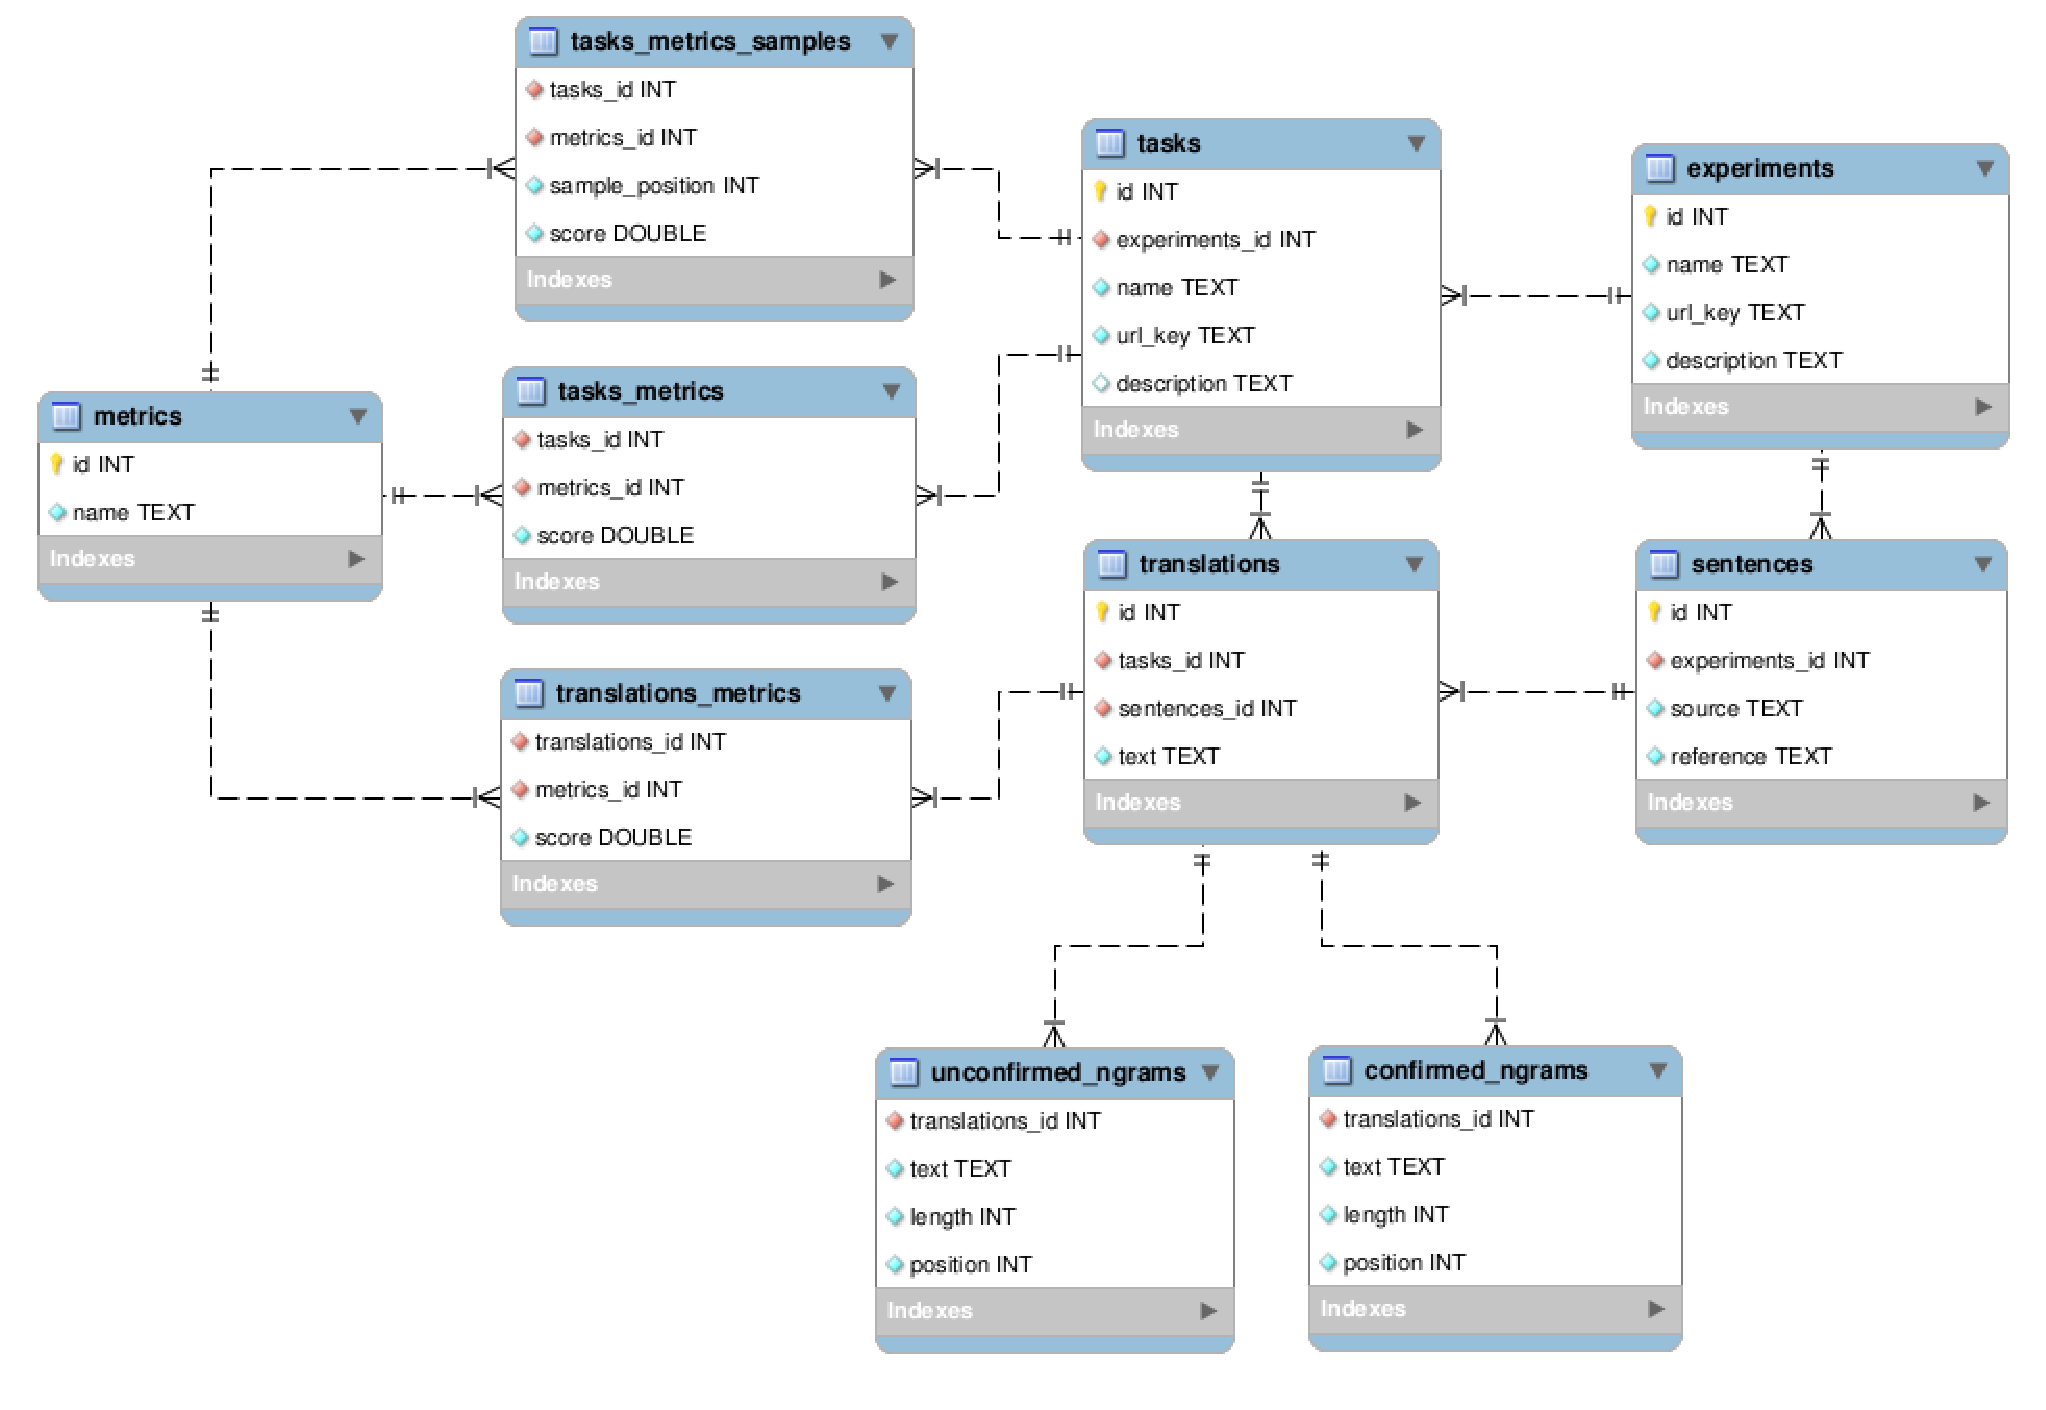
\includegraphics[width=0.8\textwidth]{img/schema.eps}
	\caption{Schéma databáze, kterou používá nástroj \mbox{MT-ComparEval}}
	\label{img:schema}
\end{figure}

\subsection{Párový bootstrap resampling}
\label{chap:bootstrap-resampling}
%% rozsirit sekci o bootstrap resamplingu
Aby na frontendu bylo možné porovnávat dva překlady pomocí párového bootstrap resamplingu,
  musí být předgenerovány náhodné vzorky.
Pro porovnání dvou překladů pomocí této metody je nutné,
  aby pro porovnávané překlady byly vzorky vygenerovány se stejnými větami.
Proto jsou pro každý experiment náhodně zafixována čísla vět,
  která budou ke generování vzorku použita.\footnote{
	Ve skutečnosti není potřeba zafixovávat čísla vět,
	při generování vzorků stačí nastavit vždy stejné jadérko pro generátor náhodných čísel.
  }
Pro takto vygenerované vzorky vět jsou spočteny všechny metriky a
  z~jejich výsledků je na frontendu vykreslen graf.

\subsection{Hledání nejvíce zlepšujících a zhoršujících \mbox{n-gramů}}
\label{chap:improving-worsening}
Jelikož zlepšujících \mbox{n-gramů} se v~překladech může nacházet velké množství,
  je třeba, aby nejvíce zlepšující \mbox{n-gramy} byly předpočítány.
Při importu tasku jsou proto předpočítány nejvíce zlepšující \mbox{n-gramy} pro porovnání daného tasku se všemi ostatními tasky,
  které se nacházejí ve stejném experimentu.
Algoritmus pro hledání nejvíce zlepšujících \mbox{n-gramů} připomíná algoritmus mergesort (viz Algoritmus \ref{alg:improving}).
Pomocí obdobného postupu se také hledají nejvíce zhoršující \mbox{n-gramy}.

\begin{algorithm}
	\begin{verbatim}
		CONFIRMED_NGRAMS_A = get all confirmed n-grams for TASK_A
		CONFIRMED_NGRAMS_B = get all confitmed n-grams for TASK_B

		while CONFIRMED_NGRAMS_A and CONFIRMED_NGRAMS_B are not empty do
		    CONFIRMED_A = first n-gram in CONFIRMED_NGRAMS_A
		    CONFIRMED_B = first n-gram in CONFIRMED_NGRAMS_B

		    if CONFIRMED_A > CONFIRMED_B then
		        set CONFIRMED_B as improving in TASK_B
		        pop first n-gram from CONFIRMED_NGRAMS_B
		    else if CONFIRMED_A < CONFIRMED_B then
		        set CONFIRMED_A as improving in TASK_A
		        pop first n-gram from CONFIRMED_NGRAMS_A
		    else then
		        pop first n-gram from CONFIRMED_NGRAMS_A
		        pop first n-gram from CONFIRMED_NGRAMS_B
		    done
		done

		while CONFIRMED_NGRAMS_A is not empty do
		    set CONFIRMED_A as improving in TASK_A
		    pop first n-gram from CONFIRMED_NGRAMS_A
		done

		while CONFIRMED_NGRAMS_B is not empty do
		    set CONFIRMED_B as improving in TASK_B
		    pop first n-gram from CONFIRMED_NGRAMS_B
		done

		choose top 10 improving n-grams for TASK_A
		choose top 10 improving n-grams for TASK_B
	\end{verbatim}

	\caption{Algoritmus pro nalezení 10 nejvíce zlepšujících \mbox{n-gramů} v~porovnávaných tascích}
	\label{alg:improving}
\end{algorithm}



%% TODO dodelat vypnuti predpocitani tasku
Protože předpočítání nejvíce zlepšujících/zhoršujících \mbox{n-gramů} pro všechny tasky může být časově náročné,
  je možné toto předpočítání v~konfiguraci jednotlivých tasků vypnout.
V~porovnání dvou tasků pak nebudou předpočítané \mbox{n-gramy} ihned k~dispozici
  a budou se muset při prvním požadavku dopočítat. 

\subsection{Logování importů}
%% přidat ukázky logů
Všechny důležité operace spojené s~importem tasků či experimentů
  (načítání konfiguračního souboru, načítání vět ze souborů,
  počítání metrik, ukládání do databáze atd.), 
  jsou logovány do souboru,
  z~kterého je možné vyčíst,
  proč nebyl některý task či experiment úspěšně importován. 


\section{REST API}
REST API je implementované v~jazyce PHP s~použitím frameworku Nette.
Toto API slouží k~předávání předpočítaných informací frontendu,
  který si je dle potřeby získává za použití AJAXu.
Api vždy vrací data ve formátu JSON,
  který lze snadno použít v~Javascriptu.
Pomocí API navíc mohou být získávána pouze data,
  která v~danou chvíli frontend potřebuje.
To znamená, že se nemusí načítat všechny věty naráz,
  ale mohou být načítány postupně,
  s~tím, jak si je uživatel prohlíží.
Stejně tak nemusí být stahována všechna data pro grafy,
  ale stačí stáhnout data pouze pro právě vybranou metriku.

Pomocí API je možné získat většinu dat pro porovnání dvou překladů,
  ať už se jedná o~dostupné metriky,
  data pro vykreslení grafů právě vybrané metriky,
  nejvíce zlepšující a zhoršující \mbox{n-gramy}
  nebo věty,
  které mohou být řazeny podle libovolné metriky.

\section{Frontend}
Na frontendu byl použit CSS framework Bootstrap\footnote{http://twitter.github.io/bootstrap/} od firmy Twitter,
  javascriptový framework AngularJS od firmy Google
  a knihovna Highcharts\footnote{http://www.highcharts.com} pro vykreslování grafů.

Na frontendu se nacházejí tři typy stránek:
\begin{itemize}
  \item seznam všech experimentů,
  \item seznam všech tasků v~daném experimentu a
  \item porovnání dvou tasků.
\end{itemize}

Na frontendu dochází k~výpisu dat, která byla předpočítána během importu jednotlivých tasků.
Pouze pozice potvrzených \mbox{n-gramů} a diff se počítají až při zobrazení jednotlivých vět.
Algoritmus, pomocí kterého se hledají pozice potvrzených \mbox{n-gramů}, byl vysvětlen v~Kapitole \ref{chap:compare}.
Způsob, jakým jsou potvrzené \mbox{n-gramy} zobrazeny, je popsán v~následující části.

\subsection{Zobrazení potvrzených \mbox{n-gramů} a diffu pomocí CSS}
Pro správné zobrazení potvrzených \mbox{n-gramů} a diffu je třeba,
  aby bylo možné u~každého tokenu určit,
  zda se nachází v~nějakém potvrzeném \mbox{n-gramu} nebo se jedná o~nepotvrzený \mbox{n-gram}.
Také je důležité,
  aby jednotlivá zvýraznění bylo možné libovolně kombinovat.
Technicky tento problém byl vyřešen pomocí CSS tříd,
  kdy každému tokenu byly přiřazeny třídy v~závislosti na informacích,
  které byly vypočítány při importu tasků.
Jednotlivé kombinace lze zapnout přiřazením příslušné třídy kořenovému elementu,
  ve~kterém se nacházejí všechny věty.

\section{Implementace vlastních metrik}
\label{chap:own-metrics}

Nástroj \mbox{MT-ComparEval} umožňuje doprogramování vlastních metrik strojového překladu.
Stačí pouze doprogramovat implementaci rozhraní \textbf{IMetrics} a
  zaregistrovat ji jako novou metriku.

Jednotlivé kroky budou v~následující části podrobně rozebrány.

\subsection{Rozhraní IMetrics}
\begin{verbatim}
interface IMetrics {
    public function init();
    public function addSentence( $reference, $translation, $meta );
    public function getScore();
}
\end{verbatim}

Rozhraní \texttt{IMetrics} představuje zapouzdření výpočtu jednotlivých strojových metrik.
Toto rozhraní umožňuje vypočítat metriku na úrovni celého dokumentu nebo jednotlivých vět.

\begin{itemize}
	\item \texttt{init()} \\
		Metoda \texttt{init} slouží k~inicializaci metriky před začátkem výpočtu.	
		Jelikož jsou instance jednotlivých metrik znovupoužívány,
		  je třeba,
		  aby byly před každým výpočtem znovu inicializovány,
		  aby se jednotlivé výpočty navzájem neovlivňovaly.

	
	\item \texttt{addSentence(\$reference, \$translation, \$meta)} \\
		Metoda \texttt{addSentence} slouží k~předání informací o~právě zpracovávané větě.
		Zároveň ihned s~tím i vrací hodnotu metriky pro danou větu.
		Parametr \texttt{\$reference} obsahuje text reference, 
                  parametr \texttt{\$translation} obsahuje text překladu a
                  parametr \texttt{\$meta} obsahuje metainformace o~větě,
                  které byly předpočítány během importu vět.
                Mezi tyto metainformace patří např. výčet potvrzených a nepotvrzených \mbox{n-gramů},
                  počet potvrzených \mbox{n-gramů} i počet \mbox{n-gramů} v~překladu.
		Tyto metainformace pak jsou použity např. při výpočtu BLEU,
		  aby se nemusely při každém počítání metriky počítat znovu.

	\item \texttt{getScore()}
		Metoda \texttt{getScore} vrací výslednou hodnotu metriky pro celý dokument.
 
\end{itemize}


\subsection{Registrace nové metriky}
Registrace nové metriky se skládá ze dvou kroků.
\begin{itemize}
	\item \textbf{uložení jména nové metriky do tabulky \texttt{metrics}} \\
		Nejprve je nutné vymyslet jméno pro novou metriku a toto jméno uložit do tabulky \texttt{metrics}. 
		Jelikož jsou všechny metriky počítány \mbox{case-sensitive} i \mbox{case-insensitive},
		  je třeba do tabulky \texttt{metrics} vložit i jméno pro \mbox{case-insensitive} hodnotu. 
		Ta je určena sufixem \texttt{-cis}.

		Vložení metriky BLEU do databáze lze provést následujícím způsobem:
		\begin{verbatim}
			$ sqlite3 app/database
			sqlite> INSERT INTO metrics (name) VALUES ('bleu');
			sqlite> INSERT INTO metrics (name) VALUES ('bleu-cis');
		\end{verbatim}

	\item \textbf{zaregistrování nové metriky v~konfiguraci aplikace} \\
		Framework Nette používá ke konfiguraci aplikací konfigurační soubory ve formátu neon.\footnote{
			Pro pochopení konfigurace je třeba přečíst http://doc.nette.org/cs/configuring\#toc-vlastni-sluzby
		}
		Nejprve je potřeba novou metriku zaregistrovat jako službu a poté přidat tuto službu konfiguraci \texttt{TasksImporteru}.
		Registraci nové metriky lze ukázat na přikladu registrace metriky Recall:


		\begin{verbatim}
			common:
			    service:
			        ...
			        bleu: Bleu
			        recall: Recall 
			        ...

			        tasksImporters:
			            class: TasksImporter(
			                ...
			                [ @bleu, @recall ]
			             )
		\end{verbatim}
\end{itemize}
